\documentclass[10pt,a4paper]{article}
\usepackage[utf8]{inputenc}
\usepackage[spanish]{babel}

\usepackage{amsmath}
\usepackage{amsfonts}
\usepackage{amssymb}
\usepackage{graphicx}
\usepackage{graphics}
\usepackage{caption}
\usepackage{subcaption}
\usepackage{listings}

\usepackage{color} %red, green, blue, yellow, cyan, magenta, black, white
\definecolor{mygreen}{RGB}{28,172,0} % color values Red, Green, Blue
\definecolor{mylilas}{RGB}{170,55,241}
\definecolor{mygray}{rgb}{0.5,0.5,0.5}
\definecolor{mymauve}{rgb}{0.58,0,0.82}
\definecolor{myblue}{rgb}{0.33,0.33,0.99}
\lstset{language=C++,%
    basicstyle=\color{red},
    breaklines=true,%
    morekeywords={matlab2tikz},
    keywordstyle=\color{blue},%
    morekeywords=[2]{1}, keywordstyle=[2]{\color{green}},
    identifierstyle=\color{black},%
    stringstyle=\color{mygreen},
    commentstyle=\color{mygray},%
    showstringspaces=false,%without this there will be a symbol in the places where there is a space
    numbers=left,%
    numberstyle={\tiny \color{mygray}},% size of the numbers
    numbersep=9pt, % this defines how far the numbers are from the text
    emph=[1]{for,end,break},emphstyle=[1]\color{blue}, %some words to emphasise
    emph=[2]{word1,word2}, emphstyle=[2]{style},    
}

\title{Facultad de Ingenieria,\\
 Universidad de Buenos Aires\\
 75.04 - Algoritmos y Programación 2\\
Trabajo Práctico nº 2}
\author{Carlos Germán Carreño Romano\\
Cristian Zózimo Aranda Cordero,\\
Federico Verstraeten}
\begin{document}

\maketitle
\newpage
\tableofcontents
\newpage
\section{Introducción}
El objetivo de este trabajo es modelar estructuras de datos.\\

\section{Diseño e Implementación}



\section{Ejecuciones}


\subsection{Compilación}

La compilación del programa se realiza por medio de un Makefile. El detalle se encuentra en la sección CODE::Makefile. Como salida, se genera un archivo ejecutable de extension.exe.

Para ejecutar el programa se necesita invocar con la siguiente línea de comandos:
\texttt{$./main_TP1.exe -i <entrada.txt> -o <salida.txt>$}
Las pruebas que se realizaron contemplan archivos correctos de entrada, y algunos ejemplos que contienen topologías inconexas y topologías con ciclos. Los resultados se adjuntan a continuación:\\
\title{\textbf{Entrada correcta}}\\
%\begin{center}
%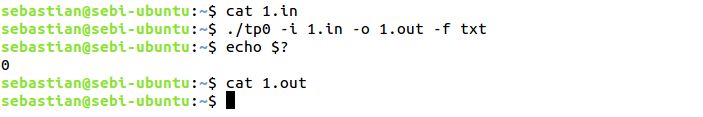
\includegraphics[scale=0.25]{Images/test1.png}\\
%\end{center}\title{Entrada de malas conexiones}\\


\section{Códigos}
%Los códigos no deben tener \textbf{\underline{texto acentuado}}.
%\subsection*{CODE::Makefile}
%\lstinputlisting{Codes/makefile}
%
%\subsection*{CODE::main}
%\lstinputlisting{Codes/main_TP1.cpp}
%
%\subsection*{CODE::Dictionary}
%\lstinputlisting{Codes/dictionary.hpp}
%\lstinputlisting{Codes/dictionary.cpp}
%
%\subsection*{CODE::NetworkElement Class}
%\lstinputlisting{Codes/NetworkElementClass.hpp}
%\lstinputlisting{Codes/NetworkElementClass.cpp}
%
%\subsection*{CODE::cmdline}
%\lstinputlisting{Codes/cmdline.h}
%\lstinputlisting{Codes/cmdline.cc}
%
%\subsection*{CODE::option}
%\lstinputlisting{Codes/options.hpp}
%\lstinputlisting{Codes/options.cpp}
%
%\subsection*{CODE::process}
%\lstinputlisting{Codes/process.hpp}
%\lstinputlisting{Codes/process.cpp}


\end{document}